% ==========================================================================
%  PFC — Planejamento de Trajetória para Robô Terrestre por meio de
%         Segmentação Semântica e Otimização em Grafos
%  Autores: Gabriel Dias Vilela e Tassandro Cavalcante Leitão
%  Instituto Militar de Engenharia — 2026
% ==========================================================================
\documentclass[
    12pt,
    openright,
    oneside,
    a4paper,
    english,
    brazil
]{abntex2}

% ── Pacotes ──────────────────────────────────────────────────────────────
\usepackage[utf8]{inputenc}
\usepackage[T1]{fontenc}
\usepackage{lmodern}
\usepackage{indentfirst}
\usepackage{graphicx}
\usepackage{microtype}
\usepackage{amsmath,amssymb}
\usepackage{algorithm}
\usepackage{algorithmic}
\usepackage{booktabs}
\usepackage{multirow}
\usepackage{hyperref}
\usepackage{float}
\usepackage{listings}
\usepackage{xcolor}
\usepackage{tikz}
\usetikzlibrary{positioning, arrows.meta, shapes.geometric, fit, backgrounds, calc}
\usepackage[brazilian,hyperpageref]{backref}
\usepackage[alf]{abntex2cite}

% ── Estilos TikZ globais para diagramas do projeto ──────────────────────
\definecolor{boxBlue}{HTML}{2E86AB}
\definecolor{boxGreen}{HTML}{56B870}
\definecolor{boxOrange}{HTML}{E07B39}
\definecolor{boxPurple}{HTML}{8E5BB5}
\definecolor{boxGray}{HTML}{6C757D}
\definecolor{bgLight}{HTML}{F4F6F8}

\tikzset{
    pipelineBox/.style={
        rectangle, rounded corners=4pt, draw=#1, fill=#1!12, line width=0.9pt,
        minimum width=2.8cm, minimum height=1.5cm, align=center,
        inner sep=4pt, font=\small\sffamily, text=black
    },
    pipelineArrow/.style={
        -{Stealth[length=3mm, width=2mm]}, line width=0.9pt, draw=boxGray
    },
    compBox/.style={
        rectangle, rounded corners=3pt, draw=#1, fill=#1!10, line width=0.7pt,
        minimum width=5.6cm, minimum height=0.9cm, align=center,
        font=\footnotesize\sffamily, text=black
    },
    compTitle/.style={
        rectangle, rounded corners=3pt, fill=#1, line width=0.7pt,
        minimum width=5.6cm, minimum height=0.95cm, align=center,
        font=\small\bfseries\sffamily, text=white
    },
    compArrow/.style={
        -{Stealth[length=2.5mm, width=1.8mm]}, line width=0.7pt, draw=#1
    }
}

% ── Configuração de listings para Python ─────────────────────────────────
\lstset{
    language=Python,
    basicstyle=\ttfamily\small,
    keywordstyle=\color{blue}\bfseries,
    stringstyle=\color{red},
    commentstyle=\color{gray}\itshape,
    numbers=left,
    numberstyle=\tiny\color{gray},
    breaklines=true,
    frame=single,
    captionpos=b,
}

% ── Dados do documento ───────────────────────────────────────────────────
\titulo{Planejamento de Trajetória para Robô Terrestre por meio de Segmentação Semântica e Otimização em Grafos}
\autor{Gabriel Dias Vilela \and Tassandro Cavalcante Leitão}
\local{Rio de Janeiro}
\data{2026}
\orientador{Claudia Marcela Justel, D.Sc.}
\coorientador{Paulo Fernando Ferreira Rosa, Ph.D.}
\instituicao{%
    MINISTÉRIO DA DEFESA\\
    EXÉRCITO BRASILEIRO\\
    DEPARTAMENTO DE CIÊNCIA E TECNOLOGIA\\
    INSTITUTO MILITAR DE ENGENHARIA\\
    CURSO DE GRADUAÇÃO EM ENGENHARIA DA COMPUTAÇÃO
}
\tipotrabalho{Projeto de Final de Curso}
\preambulo{Projeto de Final de Curso apresentado ao Curso de Graduação em Engenharia da Computação do Instituto Militar de Engenharia, como requisito parcial para a obtenção do título de Bacharel em Engenharia da Computação.}

% ==========================================================================
\begin{document}

\selectlanguage{brazil}
\frenchspacing

% ══════════════════════════════════════════════════════════════════════════
%  ELEMENTOS PRÉ-TEXTUAIS
% ══════════════════════════════════════════════════════════════════════════
\pretextual

% ── Capa ─────────────────────────────────────────────────────────────────
\begin{capa}
    \center
    \ABNTEXchapterfont

    {\normalsize
    MINISTÉRIO DA DEFESA\\
    EXÉRCITO BRASILEIRO\\
    DEPARTAMENTO DE CIÊNCIA E TECNOLOGIA\\
    INSTITUTO MILITAR DE ENGENHARIA\\
    CURSO DE GRADUAÇÃO EM ENGENHARIA DA COMPUTAÇÃO}

    \vspace*{2cm}

    {\large GABRIEL DIAS VILELA}\\
    {\large TASSANDRO CAVALCANTE LEITÃO}

    \vspace*{3cm}

    {\Large\bfseries PLANEJAMENTO DE TRAJETÓRIA PARA ROBÔ TERRESTRE POR MEIO DE SEGMENTAÇÃO SEMÂNTICA E OTIMIZAÇÃO EM GRAFOS}

    \vfill

    {\large RIO DE JANEIRO}\\
    {\large 2026}
\end{capa}

% ── Folha de rosto ───────────────────────────────────────────────────────
\begin{folhaderosto}
    \center
    {\large GABRIEL DIAS VILELA}\\
    {\large TASSANDRO CAVALCANTE LEITÃO}

    \vspace*{3cm}

    {\Large\bfseries PLANEJAMENTO DE TRAJETÓRIA PARA ROBÔ TERRESTRE POR MEIO DE SEGMENTAÇÃO SEMÂNTICA E OTIMIZAÇÃO EM GRAFOS}

    \vspace*{2cm}

    \hspace{.45\textwidth}
    \begin{minipage}{.5\textwidth}
        \imprimirpreambulo\\[1em]
        Orientador(es): Claudia Marcela Justel, D.Sc.\\
        Paulo Fernando Ferreira Rosa, Ph.D.
    \end{minipage}

    \vfill

    {\large Rio de Janeiro}\\
    {\large 2026}
\end{folhaderosto}

% ── Ficha catalográfica ─────────────────────────────────────────────────
\begin{fichacatalografica}
    \vspace*{\fill}
    \begin{center}
    {\normalsize \copyright 2026\\
    INSTITUTO MILITAR DE ENGENHARIA\\
    Praça General Tibúrcio, 80 -- Praia Vermelha\\
    Rio de Janeiro -- RJ CEP: 22290-270}
    \end{center}

    \vspace{1cm}

    \noindent Este exemplar é de propriedade do Instituto Militar de Engenharia, que poderá incluí-lo em base de dados, armazenar em computador, microfilmar ou adotar qualquer forma de arquivamento.

    É permitida a menção, reprodução parcial ou integral e a transmissão entre bibliotecas deste trabalho, sem modificação de seu texto, em qualquer meio que esteja ou venha a ser fixado, para pesquisa acadêmica, comentários e citações, desde que sem finalidade comercial e que seja feita a referência bibliográfica completa.

    Os conceitos expressos neste trabalho são de responsabilidade do(s) autor(es) e do(s) orientador(es).

    \vspace{1cm}

    \noindent
    Dias Vilela, Gabriel; Cavalcante Leitão, Tassandro.\\
    Planejamento de trajetória para robô terrestre por meio de segmentação semântica e otimização em grafos / Gabriel Dias Vilela e Tassandro Cavalcante Leitão. -- Rio de Janeiro, 2026.\\
    XX f.\\[0.5em]
    Orientador(es): Claudia Marcela Justel e Paulo Fernando Ferreira Rosa.\\[0.5em]
    Projeto de Final de Curso (graduação) -- Instituto Militar de Engenharia, Engenharia da Computação, 2026.\\[0.5em]
    1.~Veículos terrestres não tripulados. 2.~Segmentação semântica. 3.~Algoritmos baseados em grafos. 4.~Planejamento de trajetórias. 5.~Aprendizado de máquina. i.~Justel, Claudia Marcela (orient.) ii.~Ferreira Rosa, Paulo Fernando (orient.) iii.~Título
    \vspace*{\fill}
\end{fichacatalografica}

% ── Folha de aprovação ──────────────────────────────────────────────────
\begin{folhadeaprovacao}
    \center

    {\large GABRIEL DIAS VILELA}\\
    {\large TASSANDRO CAVALCANTE LEITÃO}

    \vspace{1cm}

    {\large\bfseries Planejamento de trajetória para robô terrestre por meio de segmentação semântica e otimização em grafos}

    \vspace{1cm}

    Projeto de Final de Curso apresentado ao Curso de Graduação em Engenharia da Computação do Instituto Militar de Engenharia, como requisito parcial para a obtenção do título de Bacharel em Engenharia da Computação.

    \vspace{0.5cm}

    Orientador(es): Claudia Marcela Justel e Paulo Fernando Ferreira Rosa.

    \vspace{0.5cm}

    Aprovada em \_\_\_ de \_\_\_\_\_\_\_\_\_\_\_ de 2026, pela seguinte banca examinadora:

    \vspace{1.5cm}

    \assinatura{Prof. Paulo Fernando Ferreira Rosa -- Professor do IME -- Presidente}
    \assinatura{Profa. Claudia Marcela Justel -- Professora do IME}
    \assinatura{Membro 3 -- Instituição}
    \assinatura{Membro 4 -- Instituição}
    \assinatura{Membro 5 -- Instituição}

    \vfill

    {\large Rio de Janeiro}\\
    {\large 2026}
\end{folhadeaprovacao}

% ── Dedicatória ──────────────────────────────────────────────────────────
\begin{dedicatoria}
    \vspace*{\fill}
    \centering
    \noindent
    \textit{Às nossas famílias.}
    \vspace*{\fill}
\end{dedicatoria}

% ── Agradecimentos ──────────────────────────────────────────────────────
\begin{agradecimentos}
Os agradecimentos principais são direcionados aos nossos orientadores por todo acompanhamento e ensinamentos. Agradecemos também aos autores do projeto anterior, João Vitor Camelo de Almeida e Thiago Calheiros de Souza Barbosa, cujo trabalho serviu de base e inspiração para o presente projeto.
\end{agradecimentos}

% ── Epígrafe ─────────────────────────────────────────────────────────────
\begin{epigrafe}
    \vspace*{\fill}
    \begin{flushright}
        \textit{``Não vos amoldeis às estruturas deste mundo,\\
        mas transformai-vos pela renovação da mente,\\
        a fim de distinguir qual é a vontade de Deus:\\
        o que é bom, o que Lhe é agradável, o que é perfeito.''}\\
        (Bíblia Sagrada, Romanos 12, 2)
    \end{flushright}
\end{epigrafe}

% ── Resumo ───────────────────────────────────────────────────────────────
\setlength{\absparsep}{18pt}
\begin{resumo}
Este projeto dá continuidade ao trabalho de planejamento de trajetória para veículos terrestres não tripulados desenvolvido em 2025, estendendo-o em duas frentes principais: (i)~a adoção de uma arquitetura de \textit{software} orientada a objetos e modular, organizada em cinco estágios encadeados --- ingestão de dados, pré-processamento (segmentação semântica), construção de grafos, algoritmos de caminho mínimo e pós-processamento; e (ii)~a substituição da abordagem anterior de tratamento de imagens por uma estratégia baseada em modelos de segmentação semântica pré-treinados sobre o \textit{Semantic Drone Dataset} \cite{drone_dataset}, disponibilizados em \cite{junior2024_models} (ResNet~50, ResNet~101, EfficientNet-B4 e EfficientNet-B5), que recebem imagens aéreas reais capturadas por UAV e produzem mapas de navegabilidade nos quais as regiões transitáveis são codificadas por cores específicas, conforme a metodologia consolidada em \cite{junior2025_rrt}. Os algoritmos A*, Dijkstra, BFS e DFS foram reimplementados sobre uma representação genérica de grafo, com \textit{node embeddings}, \textit{edge index} e \textit{edge embeddings}. Os caminhos calculados são, em seguida, encaminhados a um módulo de pós-processamento que produz \textit{waypoints} compatíveis com o simulador Gazebo \cite{koenig2004}, no qual a trajetória do UGV é validada antes de qualquer implantação em campo.

\textbf{Palavras-chave}: Veículos terrestres não tripulados; Segmentação semântica; Algoritmos baseados em grafos; Planejamento de trajetórias; Aprendizado de máquina; Simulador Gazebo.
\end{resumo}

% ── Abstract ─────────────────────────────────────────────────────────────
\begin{resumo}[Abstract]
\begin{otherlanguage*}{english}
This project continues the trajectory planning work for unmanned ground vehicles developed in 2025, extending it in two main directions: (i)~an object-oriented, modular software architecture organized into five chained stages---data ingestion, preprocessing (semantic segmentation), graph construction, shortest-path algorithms, and post-processing; and (ii)~the replacement of the previous color-based image processing approach by a strategy that leverages semantic segmentation models pre-trained on the \emph{Semantic Drone Dataset} \cite{drone_dataset}, released in \cite{junior2024_models} (ResNet~50, ResNet~101, EfficientNet-B4 and EfficientNet-B5), which take aerial RGB images acquired by a UAV and produce navigability maps in which traversable regions are encoded by specific colors, following the methodology consolidated in \cite{junior2025_rrt}. The A*, Dijkstra, BFS, and DFS algorithms were reimplemented over a generic graph representation with node embeddings, edge indices, and edge embeddings. The computed paths are then forwarded to a post-processing module that produces waypoints compatible with the Gazebo simulator \cite{koenig2004}, where the UGV trajectory is validated before any field deployment.

\textbf{Keywords}: Unmanned ground vehicles; Semantic segmentation; Graph-based algorithms; Trajectory planning; Machine learning; Gazebo simulator.
\end{otherlanguage*}
\end{resumo}

% ── Listas ───────────────────────────────────────────────────────────────
\pdfbookmark[0]{\listfigurename}{lof}
\listoffigures*
\cleardoublepage

\pdfbookmark[0]{\listtablename}{lot}
\listoftables*
\cleardoublepage

% ── Lista de abreviaturas ───────────────────────────────────────────────
\begin{siglas}
    \item[BFS] Breadth-First Search
    \item[CNN] Convolutional Neural Network
    \item[CTEx] Centro Tecnológico do Exército
    \item[DFS] Depth-First Search
    \item[EB] Exército Brasileiro
    \item[IA] Inteligência Artificial
    \item[mIoU] Mean Intersection over Union
    \item[OOP] Object-Oriented Programming
    \item[ROS] Robot Operating System
    \item[RRT] Rapidly-exploring Random Tree
    \item[SVTRP] Sistemas de Veículos Terrestres Remotamente Pilotados
    \item[UAV] Unmanned Aerial Vehicle
    \item[UGV] Unmanned Ground Vehicle
\end{siglas}

% ── Sumário ──────────────────────────────────────────────────────────────
\pdfbookmark[0]{\contentsname}{toc}
\tableofcontents*
\cleardoublepage

% ══════════════════════════════════════════════════════════════════════════
%  ELEMENTOS TEXTUAIS
% ══════════════════════════════════════════════════════════════════════════
\textual

% ======================================================================
\chapter{INTRODUÇÃO}
% ======================================================================

Os avanços tecnológicos envolvendo visão computacional, eletrônica e inteligência artificial, entre outras áreas correlatas, impulsionaram a tendência de desenvolvimento e uso de ferramentas que automatizam as disputas em ambientes de combate. Nesse sentido, com a possibilidade de aumentar a eficácia operacional e reduzir a participação e desgaste humano --- física, cognitiva e psicologicamente --- no campo de batalha, a integração de robôs autônomos nesses cenários de confronto é iminente e torna-se motivo de vantagem tática e estratégica.

Em relação à autonomia desses sistemas, o planejamento de trajetória de robôs terrestres é uma das tarefas essenciais a ser realizada e ela se encontra dentro de um escopo multidisciplinar que inclui conhecimentos em diversas áreas de grande complexidade, como a robótica e a teoria dos grafos. Essas disciplinas convergem na modelagem do cenário de combate como um grafo, no qual os nós representam as posições transitáveis pelos robôs no mapa e as arestas definem os caminhos. Dessa maneira, algoritmos de busca e otimização são ferramentas que guiam o planejamento das possíveis rotas, auxiliando na coordenação entre pontos e adaptação aos obstáculos.

A pesquisa ``Cooperação Entre Plataformas Terrestres e Aéreas para Aquisição, Rastreamento e Perseguição de Alvos, Utilizando Visão Computacional e Inteligência Artificial'' \cite{junior2024} que se encontra em fase de desenvolvimento no laboratório LIARC, iniciada em 2023 pelo Major Fábio Luiz Junior, aborda o emprego de plataformas robóticas aéreas (UAV) e terrestres (UGV) em ambientes de batalha e como essas duas estruturas podem trabalhar em conjunto para otimizar e ampliar o poder de ataque e estratégico militar.

\subsection*{Contribuições do Projeto Anterior}

O presente projeto é uma continuação direta do trabalho ``Planejamento de Trajetória para Robô Terrestre, Utilizando Otimização em Grafos'', desenvolvido em 2025 por Camelo de Almeida e Calheiros de Souza Barbosa \cite{camelo2025}. Naquele trabalho, os autores propuseram uma abordagem baseada em grafos para o planejamento de caminhos sobre imagens aéreas segmentadas semanticamente, implementando os algoritmos de Dijkstra e A* e comparando-os com o algoritmo estocástico RRT.

As principais conclusões do projeto de 2025 foram:
\begin{itemize}
    \item Os algoritmos baseados em grafos (Dijkstra e A*) apresentaram desempenho mais consistente, confiável e previsível em relação ao RRT, destacando-se pelo determinismo e pela garantia de otimalidade das soluções;
    \item O algoritmo A* mostrou-se ligeiramente mais rápido que o Dijkstra, explorando um menor número de nós, sendo considerado mais adequado ao problema proposto;
    \item A inserção de pesos nas arestas do grafo, com base na proximidade a obstáculos, produziu caminhos mais realistas que se distanciam de regiões de risco, sem impacto significativo no tempo de execução;
    \item O RRT apresentou dificuldades em imagens com áreas transitáveis estreitas, excedendo o tempo limite em dois dos cinco cenários testados;
    \item A abordagem proposta, ao integrar segmentação semântica de imagens e planejamento baseado em grafos, constitui uma alternativa promissora para aplicações em veículos autônomos.
\end{itemize}

Como perspectivas futuras, aquele trabalho identificou a necessidade de: (i)~tratamento de ambientes dinâmicos com algoritmos como o D*; (ii)~avaliação do impacto do uso de grafos em situações de composição de imagens em tempo real; e (iii)~extensão da segmentação semântica para lidar com uma maior variedade de terrenos.

É neste último ponto que o presente projeto se concentra com maior ênfase, ao incorporar técnicas modernas de segmentação semântica baseadas em aprendizado profundo. Em vez do tratamento de imagens por meio de filtros e segmentação por cor adotado anteriormente, o presente trabalho utiliza diretamente os modelos pré-treinados disponibilizados em \cite{junior2024_models}, originalmente desenvolvidos como parte da pesquisa de doutorado de Junior \cite{junior2024} e treinados sobre o \emph{Semantic Drone Dataset}~\cite{drone_dataset}. Esses modelos, baseados em arquiteturas como ResNet~50, ResNet~101, EfficientNet-B4 e EfficientNet-B5, são capazes de classificar uma ampla gama de tipos de terreno diretamente a partir de imagens RGB reais de drones, gerando mapas de navegabilidade no formato consolidado em \cite{junior2025_rrt} --- ou seja, imagens nas quais áreas transitáveis aparecem em cores específicas, prontas para serem convertidas em grafos. Além disso, propõe-se uma arquitetura de \textit{software} modular e extensível, capaz de acomodar facilmente novos algoritmos, modelos de segmentação e métodos de pós-processamento.

% ── 1.1 ──────────────────────────────────────────────────────────────────
\section{Motivação e Justificativa}

O presente projeto busca dar continuidade e aprofundar o estudo de planejamento de rotas abordado em \cite{camelo2025} e \cite{junior2024} e, que por sua vez, poderá ser aproveitado e aplicado no projeto estratégico ``Sistemas de Veículos Terrestres Remotamente Pilotados'' (SVTRP), conduzido pelo Centro Tecnológico do Exército (CTEx), visando a uma potencialização de seu funcionamento.

O projeto anterior demonstrou a viabilidade da abordagem baseada em grafos, porém dependia de imagens previamente segmentadas por redes neurais externas. A necessidade de integrar o processo de segmentação diretamente no \textit{pipeline} de planejamento, utilizando modelos especializados em imagens de drones e capazes de lidar com a diversidade de terrenos encontrados em cenários reais, constitui a principal motivação deste trabalho. A adoção dos modelos pré-treinados disponibilizados em \cite{junior2024_models} permite reutilizar diretamente o conhecimento já validado em pesquisa anterior do laboratório \cite{junior2024}, evitando o re-treinamento e mantendo coerência com a linha de trabalho do CTEx.

Adicionalmente, em relação ao projeto anterior \cite{camelo2025}, a adoção de uma arquitetura modular orientada a objetos constitui uma melhoria estrutural significativa: ao definir interfaces abstratas para cada estágio do \textit{pipeline}, o sistema possibilita a fácil incorporação de novos algoritmos, representações de grafos e métodos de pré-processamento, sem necessidade de reescrita do restante do código. Por fim, motivada pelo objetivo de validar os caminhos calculados antes de qualquer implantação em campo, esta extensão prevê o encaminhamento dos \textit{waypoints} produzidos pelo módulo de pós-processamento ao simulador Gazebo \cite{koenig2004}, no qual a trajetória do UGV pode ser executada em um ambiente sintético controlado.

% ── 1.2 ──────────────────────────────────────────────────────────────────
\section{Objetivos}

O principal objetivo deste Projeto de Final de Curso consiste em estender o sistema de planejamento de trajetória desenvolvido em \cite{camelo2025}, incorporando segmentação semântica automatizada e uma arquitetura de \textit{software} modular, a fim de fazer uma estrutura que possa ser utilizada para simulação em ambiente virtual, visando a validação dos métodos de processamento estudados. 

Para atingir o objetivo principal, foram definidos os seguintes objetivos específicos:
\begin{itemize}
    \item Projetar e implementar uma arquitetura orientada a objetos composta por cinco módulos encadeados: ingestão de dados, pré-processamento (segmentação semântica), construção de grafos, algoritmos e pós-processamento;
    \item Integrar os modelos de segmentação semântica pré-treinados disponibilizados em \cite{junior2024_models} (ResNet~50, ResNet~101, EfficientNet-B4 e EfficientNet-B5) para identificação automática de regiões transitáveis em imagens aéreas reais, gerando mapas de navegabilidade no formato adotado em \cite{junior2025_rrt};
    \item Executar testes comparativos sobre imagens RGB reais obtidas por drone.
    \item Encaminhar os \textit{waypoints} produzidos pelo pós-processamento ao simulador Gazebo \cite{koenig2004}, viabilizando a avaliação da trajetória em um UGV simulado; e
\end{itemize}

% ── 1.3 ──────────────────────────────────────────────────────────────────
\section{Metodologia}

Visando alcançar os objetivos propostos, a metodologia adotada consiste nas seguintes etapas:

Inicialmente, foi conduzida uma revisão do projeto anterior \cite{camelo2025} e da literatura relacionada a segmentação semântica de imagens aéreas e planejamento de trajetórias.

Em seguida, projetou-se a arquitetura modular do sistema, definindo interfaces abstratas (\textit{Abstract Base Classes}) e padrões de fábrica (\textit{Factory Pattern}) para cada estágio do \textit{pipeline}: \texttt{data\_ingestion}, \texttt{preprocessing}, \texttt{graph\_parsing}, \texttt{algorithm} e \texttt{post\_processing}.

Na etapa de implementação, os algoritmos A*, Dijkstra, BFS e DFS foram reimplementados sobre a nova representação genérica de grafo, com interfaces padronizadas que desacoplam o algoritmo da estrutura de dados subjacente.

Os caminhos resultantes são, então, convertidos em \textit{waypoints} pelo módulo de pós-processamento e encaminhados ao simulador Gazebo \cite{koenig2004}, no qual a trajetória pode ser executada por um UGV simulado, permitindo avaliar de forma realista o desempenho da solução proposta antes de qualquer implantação em campo.

Por fim, foram executados testes sobre imagens RGB reais obtidas por drone, comparando os resultados dos diferentes modelos de segmentação e algoritmos de planejamento.

% ── 1.4 ──────────────────────────────────────────────────────────────────
\section{Estrutura}

Este documento está organizado da seguinte forma:

No Capítulo~2, são apresentados os conceitos preliminares que servirão de base para o desenvolvimento do projeto, incluindo fundamentos de grafos, algoritmos de caminhos mínimos e segmentação semântica.

No Capítulo~3, descreve-se a arquitetura do sistema proposto, detalhando cada módulo da \textit{pipeline}, os modelos de segmentação utilizados e a construção dos grafos.

O Capítulo~4 é dedicado à apresentação e discussão dos resultados experimentais, com a comparação do desempenho dos pré-processadores e algoritmos.

No Capítulo~5, são apresentadas as conclusões do trabalho, bem como sugestões de possíveis extensões futuras.

Por fim, o Capítulo~6 apresenta o cronograma detalhado das atividades realizadas ao longo do projeto.

% ======================================================================
\chapter{CONCEITOS PRELIMINARES}
% ======================================================================

Neste capítulo, apresentamos os conceitos fundamentais necessários para a compreensão do projeto. Além dos tópicos já abordados no projeto anterior \cite{camelo2025} --- veículos terrestres autônomos, planejamento de caminhos, grafos e algoritmos clássicos --- introduzimos conceitos de segmentação semântica e processamento de imagens que fundamentam as contribuições deste trabalho.

% ── 2.1 ──────────────────────────────────────────────────────────────────
\section{Veículos Terrestres Autônomos}

Segundo \cite{finn2010}, um veículo terrestre autônomo (UGV) é um sistema robótico complexo e multidisciplinar, com participação ostensiva das engenharias mecânica, da computação e eletrônica. Este sistema tem como objetivo navegar pelo terreno de forma autônoma, sem a necessidade de intervenção por um operador externo, e executar determinada tarefa. Nos últimos anos, evidencia-se grande crescimento nas aplicações de UGVs, desde aplicações civis até aplicações militares.

% ── 2.2 ──────────────────────────────────────────────────────────────────
\section{Planejamento de Caminhos}

O planejamento de caminhos é considerado um desafio crítico em Inteligência Artificial e essencial para o movimento autônomo de todos os sistemas inteligentes, como veículos terrestres \cite{madridano2021}. O planejamento pode ser categorizado como global (estático), quando toda a informação sobre o ambiente é conhecida, ou local (dinâmico), quando o ambiente é parcialmente desconhecido \cite{chen2020}. Neste trabalho, abordamos o planejamento de caminhos globais.

% ── 2.3 ──────────────────────────────────────────────────────────────────
\section{Grafos}

Um grafo $G = (V, E)$ consiste em um conjunto de vértices $V = \{v_1, v_2, \ldots\}$ e um conjunto de arestas $E = \{e_1, e_2, \ldots\}$, tal que cada aresta é identificada com um par de vértices $(v_i, v_j)$ \cite{chen1997}. Podemos classificar os grafos como ponderados, caso suas arestas possuam pesos associados, ou não ponderados, caso contrário.

Neste projeto, adotamos uma representação de grafo mais rica do que a utilizada no projeto anterior, incluindo:
\begin{itemize}
    \item \textbf{\textit{Node embeddings}}: vetor $(x, y, w)$ para cada nó, contendo coordenadas espaciais e peso de transitabilidade;
    \item \textbf{\textit{Edge index}}: tensor de dimensão $(2, |E|)$ com os pares (origem, destino) de cada aresta, seguindo a convenção do PyTorch Geometric;
    \item \textbf{\textit{Edge embeddings}}: vetor $(c_w, d_u)$ para cada aresta, com custo ponderado e distância euclidiana.
\end{itemize}

% ── 2.4 ──────────────────────────────────────────────────────────────────
\section{Algoritmos de Caminhos Mínimos em Grafos}

A definição de caminho mínimo entre dois vértices apoia-se em duas noções básicas da teoria dos grafos~\cite{deo2016, chen1997}. Um \emph{caminho} de um vértice $u$ para um vértice $v$ em um grafo $G = (V, E)$ é uma sequência alternada de vértices e arestas
\[
P = (v_0, e_1, v_1, e_2, v_2, \ldots, e_k, v_k),
\]
com $v_0 = u$, $v_k = v$, $e_i = (v_{i-1}, v_i) \in E$ para todo $i$ e sem repetição de vértices. O \emph{comprimento} do caminho $P$ em um grafo ponderado é a soma dos pesos das suas arestas:
\[
\ell(P) = \sum_{i=1}^{k} w(e_i),
\]
onde $w : E \to \mathbb{R}_{\geq 0}$ é a função de pesos do grafo. No caso não ponderado, define-se $w(e_i) = 1$ para toda aresta, de modo que o comprimento coincide com o número de arestas do caminho.

O \emph{problema do caminho mínimo} entre $u$ e $v$ consiste, então, em determinar um caminho $P^\ast$ tal que
\[
\ell(P^\ast) = \min \{\, \ell(P) : P \text{ é caminho de } u \text{ a } v \,\}.
\]
No contexto deste projeto, o grafo é construído a partir do mapa de navegabilidade gerado pela segmentação semântica, e o caminho mínimo corresponde à trajetória de menor custo entre o ponto inicial e o ponto final escolhidos pelo operador.

A seguir, são apresentados os quatro algoritmos clássicos implementados neste projeto.

\subsection{Breadth-First Search (BFS)}

A BFS é um algoritmo que permite percorrer vértices e arestas em grafos~\cite{cormen2009, moore1959}. Iniciando o percurso em um nó denominado fonte, a busca se expande visitando os nós em uma mesma profundidade antes de avançar. Sua particularidade --- buscar em largura --- permite determinar caminhos mínimos em grafos não ponderados de maneira eficiente, com complexidade $O(|V| + |E|)$. Por essa razão, a BFS serve de fundação para diversos outros algoritmos em grafos~\cite{beamer2013}.

\subsection{Depth-First Search (DFS)}

Diferentemente da BFS, a DFS \cite{cormen2009} explora o grafo percorrendo cada ramo o mais profundamente possível antes de retroceder. Embora não garanta encontrar o caminho mínimo, é útil em diversas aplicações em que a existência de qualquer caminho é mais relevante que sua otimalidade --- por exemplo, determinar a conexidade do grafo. Por essas razões, a DFS é incluída neste trabalho como base de comparação para os demais algoritmos.

\subsection{Algoritmo de Dijkstra}

O algoritmo de Dijkstra \cite{dijkstra1959} encontra o caminho mínimo em grafos com pesos não negativos, construindo os caminhos mínimos de forma iterativa, a partir da fonte e na ordem crescente de distância. A cada iteração, seleciona-se o vértice ainda não processado com menor distância acumulada para ser expandido, atualizando-se as estimativas de seus vizinhos.

\subsection{Algoritmo A*}

O algoritmo A* \cite{hart1968} é um algoritmo de busca informada que utiliza uma função de avaliação $f(n) = g(n) + h(n)$, onde $g(n)$ é o custo do caminho da fonte até $n$ e $h(n)$ é uma estimativa heurística do custo restante até o destino. Por se basear em uma estimativa heurística do custo até o objetivo, o A* é, em geral, um algoritmo aproximado: a qualidade da solução depende da heurística utilizada e, no caso geral, não há garantias de mínimo global. Para uma heurística admissível $h$ --- isto é, que nunca superestime o custo real até o objetivo ---, o A* recupera essa propriedade e garante otimalidade, explorando o menor número necessário de nós. Neste projeto, utiliza-se a distância euclidiana como heurística, que é admissível para grafos em grade com pesos não negativos.

% ── 2.5 ──────────────────────────────────────────────────────────────────
\section{Segmentação Semântica e Identificação de Áreas Transitáveis}
\label{sec:segmentacao}

A segmentação semântica consiste em atribuir uma classe (rótulo) a cada pixel de uma imagem. Diferentemente da classificação de imagens, que atribui um rótulo único à imagem inteira, a segmentação semântica produz um mapa denso de classes com a mesma resolução da imagem de entrada. No contexto deste projeto, a segmentação semântica é utilizada para identificar automaticamente as regiões transitáveis do terreno a partir de imagens aéreas reais, em substituição às abordagens baseadas em segmentação por cor ou em modelos genéricos de propósito amplo.

Diferentemente do projeto anterior \cite{camelo2025}, no qual eram exploradas estratégias de segmentação por limiarização no espaço HSV, optou-se neste trabalho por uma abordagem baseada nos modelos pré-treinados disponibilizados em \cite{junior2024_models}. Esses modelos foram desenvolvidos no âmbito da pesquisa de Junior~\cite{junior2024} e são treinados especificamente sobre o \emph{Semantic Drone Dataset} \cite{drone_dataset}, conjunto composto por imagens aéreas anotadas pixel a pixel para a tarefa de identificação de áreas transitáveis e não transitáveis.

\subsection{Modelos Pré-treinados Adotados}

O repositório \cite{junior2024_models} disponibiliza modelos de segmentação semântica avaliados no conjunto de teste do \emph{Semantic Drone Dataset} em termos de \emph{Mean Intersection over Union} (mIoU) e acurácia por pixel, conforme apresentado na Tabela~\ref{tab:modelos_segmentacao}:

\begin{table}[H]
    \centering
    \caption{Modelos de segmentação semântica disponibilizados em \cite{junior2024_models}.}
    \label{tab:modelos_segmentacao}
    \begin{tabular}{lcc}
        \toprule
        \textbf{Modelo} & \textbf{mIoU} & \textbf{Acurácia} \\
        \midrule
        ResNet~50        & 0,3933 & 0,8244 \\
        ResNet~101       & 0,4032 & 0,8720 \\
        EfficientNet-B4  & 0,5012 & 0,9120 \\
        EfficientNet-B5  & 0,4819 & 0,9025 \\
        \bottomrule
    \end{tabular}
\end{table}

Os modelos seguem a arquitetura U-Net, com diferentes \textit{backbones} convolucionais (ResNet~50 e ResNet~101) e baseados em redes mais modernas com escalonamento composto (EfficientNet-B4 e B5)~\cite{junior2024}. A escolha do modelo a ser utilizado em tempo de execução é, portanto, um hiperparâmetro do \textit{pipeline}, permitindo equilibrar acurácia e tempo de inferência conforme a aplicação.

\subsection{Geração do Mapa de Navegabilidade}

A saída da segmentação é processada para gerar um \emph{mapa de navegabilidade} no formato consolidado em \cite{junior2025_rrt}: uma imagem na qual as regiões transitáveis recebem cores específicas e bem definidas, enquanto as regiões não transitáveis (vegetação, edificações, obstáculos) recebem cores distintas. Esse mapa serve como entrada direta para o módulo de construção de grafos, que converte cada pixel transitável em um nó e estabelece arestas entre vizinhos imediatos. Em particular, neste trabalho adota-se o mesmo critério de \cite{junior2025_rrt}: as áreas transitáveis são representadas pelas cores BGR $(84, 1, 68)$ e $(0, 0, 255)$, e a verificação de colisão entre dois pontos é feita inspecionando as cores ao longo da reta que os conecta.

% ── 2.6 ──────────────────────────────────────────────────────────────────
\section{Pré-processamento e Pós-processamento de Máscaras}

Pelo fato de os modelos adotados \cite{junior2024_models} terem sido treinados especificamente sobre imagens aéreas do \emph{Semantic Drone Dataset}~\cite{drone_dataset}, o pré-processamento sobre as imagens RGB de entrada é mantido reduzido ao mínimo necessário: redimensionamento para a resolução esperada pela rede, conversão para o tensor de entrada e normalização estatística com a média e o desvio-padrão utilizados durante o treinamento. Não são empregadas, portanto, etapas adicionais de equalização de histograma específicas, uma vez que o próprio conjunto de treinamento já contempla variações de iluminação e cobertura de sombras.

Após a inferência da rede, é aplicado um pós-processamento sobre a máscara de classes, com o objetivo de converter a saída pixel a pixel em um mapa de navegabilidade limpo e adequado à conversão em grafo. Esse pós-processamento compreende: (i)~o agrupamento das classes do \emph{Semantic Drone Dataset} em duas categorias --- transitável e não transitável --- segundo critérios herdados de \cite{junior2024}; (ii)~operações morfológicas de fechamento e abertura, com elementos estruturantes adequados à resolução da imagem, para suavizar bordas ruidosas e fechar pequenas falhas; e (iii)~a remoção de componentes conexos de área inferior a um limiar mínimo, eliminando ``ilhas'' espúrias da segmentação. O resultado é uma máscara binária estável, à qual se aplica, por fim, a paleta de cores adotada em \cite{junior2025_rrt} para a geração do mapa de navegabilidade descrito na Seção~\ref{sec:segmentacao}.

% ── 2.7 ──────────────────────────────────────────────────────────────────
\section{Simulador Gazebo}
\label{sec:gazebo}

O Gazebo \cite{koenig2004} é um simulador robótico de código aberto amplamente utilizado pela comunidade de robótica móvel, com integração nativa ao \emph{Robot Operating System} (ROS). Ele permite modelar com elevado grau de fidelidade a dinâmica de veículos, sensores embarcados e o ambiente de operação --- incluindo terrenos, obstáculos e fontes de luz --- antes de qualquer implantação em campo. Em sistemas de UGVs, o Gazebo é tipicamente empregado para validar pilhas de navegação completas, expondo as mesmas interfaces (tópicos ROS, mensagens \texttt{nav\_msgs/Path}, etc.) que seriam utilizadas em um robô real.

No \textit{pipeline} proposto neste trabalho, o Gazebo ocupa o último estágio do fluxo: o caminho mínimo calculado pelos algoritmos é entregue ao módulo de pós-processamento, que o converte em uma sequência de \textit{waypoints}; esses \textit{waypoints} são, então, encaminhados ao Gazebo para que se avalie como a trajetória se comportaria em um UGV simulado, considerando sua dinâmica e os obstáculos do mundo virtual. Dessa forma, o simulador funciona como elo entre a saída do planejamento e o veículo físico, oferecendo uma camada adicional de validação dos caminhos produzidos pelo sistema antes da execução em campo.

% ======================================================================
\chapter{METODOLOGIA}
% ======================================================================

No presente capítulo, apresentamos a arquitetura do sistema proposto, detalhando cada módulo da \textit{pipeline}, os modelos de segmentação semântica utilizados e a construção dos grafos.

% ── 4.1 ──────────────────────────────────────────────────────────────────
\section{Arquitetura do Sistema}

O sistema foi projetado seguindo princípios de orientação a objetos, com cinco módulos independentes e encadeados, cada um definido por interfaces abstratas e instanciado por fábricas (\textit{Factory Pattern}):

\begin{enumerate}
    \item \textbf{\texttt{data\_ingestion}}: responsável pela ingestão e estruturação dos dados brutos. Define uma interface genérica (\texttt{IngestedData}) com especialização para imagens (\texttt{ImageIngestedData}) capturadas pelo UAV;
    \item \textbf{\texttt{preprocessing}}: aplica a segmentação semântica sobre a imagem ingerida, identificando os pixels transitáveis (\textit{walkable paths}) e produzindo um \texttt{SegmentedImageData} enriquecido com a máscara de navegabilidade. A interface abstrata \texttt{PreProcessor} permite o intercâmbio entre diferentes modelos sem afetar os demais módulos --- neste trabalho, é utilizada a implementação que executa os modelos pré-treinados de \cite{junior2024_models} (treinados sobre o \emph{Semantic Drone Dataset}~\cite{drone_dataset}) e gera o mapa de navegabilidade segundo o formato consolidado em \cite{junior2025_rrt};
    \item \textbf{\texttt{graph\_parsing}}: converte o mapa de navegabilidade produzido pelo \texttt{preprocessing} em uma estrutura de grafo genérica (\texttt{Graph}), com \textit{node embeddings}, \textit{edge index} e \textit{edge embeddings};
    \item \textbf{\texttt{algorithm}}: executa algoritmos de caminho mínimo sobre o grafo, retornando um \texttt{PathResult} padronizado com a sequência de nós, custo total e metadados;
    \item \textbf{\texttt{post\_processing}}: converte o resultado do algoritmo em dados utilizáveis pelo robô (\texttt{RobotPath}) ou em visualizações anotadas sobre a imagem original, produzindo a saída para a simulação da trajetória do UGV no Gazebo.
\end{enumerate}

Cada módulo possui um arquivo \texttt{interfaces.py} com classes abstratas, \texttt{entities.py} com dataclasses, \texttt{index.py} com a fábrica de registro, e um \texttt{\_\_init\_\_.py} com as exportações públicas.

A Figura~\ref{fig:pipeline} ilustra o \textit{pipeline} completo, identificando cada um dos cinco módulos pelo nome do respectivo pacote de código (\texttt{data\_ingestion}, \texttt{preprocessing}, \texttt{graph\_parsing}, \texttt{algorithm} e \texttt{post\_processing}), além da entrada (imagem RGB do UAV) e do simulador externo Gazebo, que não integra o sistema, mas recebe os \textit{waypoints} para validação.

\begin{figure}[H]
    \centering
    \resizebox{\textwidth}{!}{%
    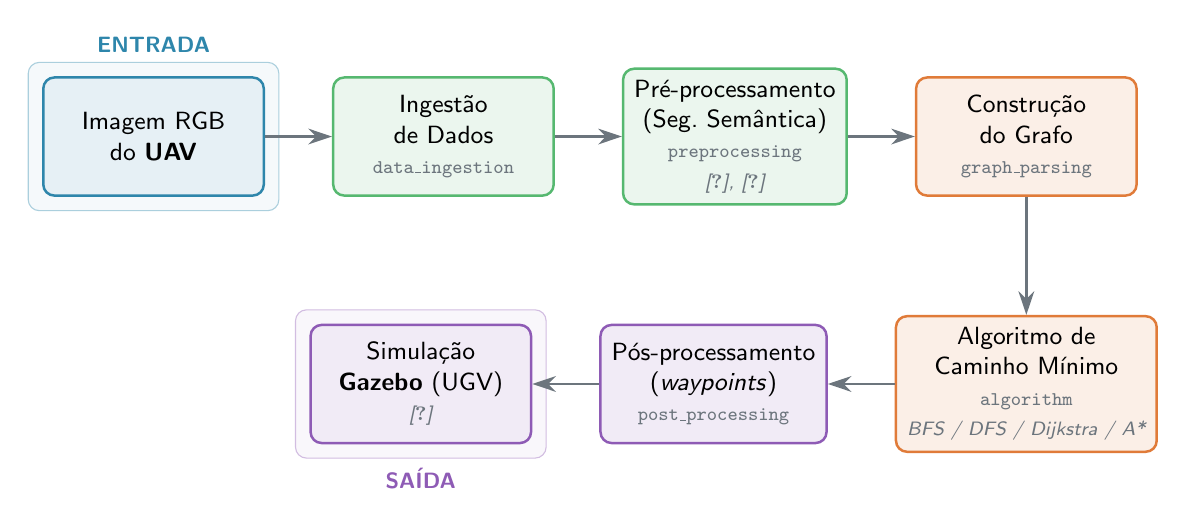
\begin{tikzpicture}[
        node distance=0.85cm and 0.85cm,
        every node/.append style={font=\small\sffamily}
    ]

        % ── Linha 1: Entrada -> Módulos 1, 2, 3 ──────────────────────────
        \node[pipelineBox=boxBlue]                    (img)
            {Imagem RGB \\ do \textbf{UAV}};
        \node[pipelineBox=boxGreen,  right=of img]    (ingest)
            {Ingestão \\ de Dados \\
             {\scriptsize\color{boxGray}\texttt{data\_ingestion}}};
        \node[pipelineBox=boxGreen,  right=of ingest] (pre)
            {Pré-processamento \\ (Seg.\ Semântica) \\
             {\scriptsize\color{boxGray}\texttt{preprocessing}} \\
             {\scriptsize\itshape\color{boxGray}\cite{junior2024_models}, \cite{junior2025_rrt}}};
        \node[pipelineBox=boxOrange, right=of pre]    (graph)
            {Construção \\ do Grafo \\
             {\scriptsize\color{boxGray}\texttt{graph\_parsing}}};

        % ── Linha 2: Módulos 4, 5 -> Saída ───────────────────────────────
        \node[pipelineBox=boxOrange, below=1.5cm of graph] (algo)
            {Algoritmo de \\ Caminho Mínimo \\
             {\scriptsize\color{boxGray}\texttt{algorithm}} \\
             {\scriptsize\itshape\color{boxGray}BFS / DFS / Dijkstra / A*}};
        \node[pipelineBox=boxPurple, left=of algo]    (post)
            {Pós-processamento \\ (\textit{waypoints}) \\
             {\scriptsize\color{boxGray}\texttt{post\_processing}}};
        \node[pipelineBox=boxPurple, left=of post]    (gz)
            {Simulação \\ \textbf{Gazebo} (UGV) \\
             {\scriptsize\itshape\color{boxGray}\cite{koenig2004}}};

        % ── Setas linha 1 ────────────────────────────────────────────────
        \draw[pipelineArrow] (img)    -- (ingest);
        \draw[pipelineArrow] (ingest) -- (pre);
        \draw[pipelineArrow] (pre)    -- (graph);

        % ── Conexão linha 1 -> linha 2 ───────────────────────────────────
        \draw[pipelineArrow] (graph.south) -- (algo.north);

        % ── Setas linha 2 (direita -> esquerda) ──────────────────────────
        \draw[pipelineArrow] (algo) -- (post);
        \draw[pipelineArrow] (post) -- (gz);

        % ── Rótulos de "entrada" e "saída" ───────────────────────────────
        \node[font=\footnotesize\sffamily\bfseries, text=boxBlue,
              anchor=south, above=0.18cm of img.north]
            {ENTRADA};
        \node[font=\footnotesize\sffamily\bfseries, text=boxPurple,
              anchor=north, below=0.18cm of gz.south]
            {SAÍDA};

        % ── Faixa de fundo destacando entrada e saída ────────────────────
        \begin{scope}[on background layer]
            \node[draw=boxBlue!40, fill=boxBlue!5, rounded corners=4pt,
                  fit=(img), inner sep=5pt] {};
            \node[draw=boxPurple!40, fill=boxPurple!5, rounded corners=4pt,
                  fit=(gz), inner sep=5pt] {};
        \end{scope}

    \end{tikzpicture}}
    \caption{Pipeline do sistema proposto com os cinco módulos (caixas verdes/laranja/roxo identificadas pelo nome do pacote): \texttt{data\_ingestion}, \texttt{preprocessing}, \texttt{graph\_parsing}, \texttt{algorithm} e \texttt{post\_processing}. A imagem RGB (entrada) e o Gazebo (saída) são elementos externos ao sistema.}
    \label{fig:pipeline}
\end{figure}

\subsection{Diferenças em Relação ao PFC 2025}
\label{subsec:diferencas_pfc2025}

Em relação ao trabalho de Camelo de Almeida e Calheiros de Souza Barbosa~\cite{camelo2025}, a arquitetura proposta neste projeto difere principalmente quanto à organização do código e ao acoplamento entre etapas. No PFC 2025, as funcionalidades de leitura de imagem, segmentação por cor, construção do grafo e execução dos algoritmos eram fortemente acopladas em \textit{scripts} sequenciais, dificultando a substituição de qualquer uma das etapas. Na proposta atual, cada etapa é encapsulada em uma classe abstrata, com fábricas dedicadas e estruturas de dados padronizadas (\texttt{IngestedData}, \texttt{Graph}, \texttt{PathResult}, \texttt{RobotPath}), permitindo a troca independente de modelos de segmentação, representações de grafo, algoritmos de caminho mínimo e formatos de saída.

A Figura~\ref{fig:comparacao_arquitetura} resume as principais diferenças estruturais entre o código do PFC 2025 e a nova proposta.

\begin{figure}[H]
    \centering
    \resizebox{\textwidth}{!}{%
    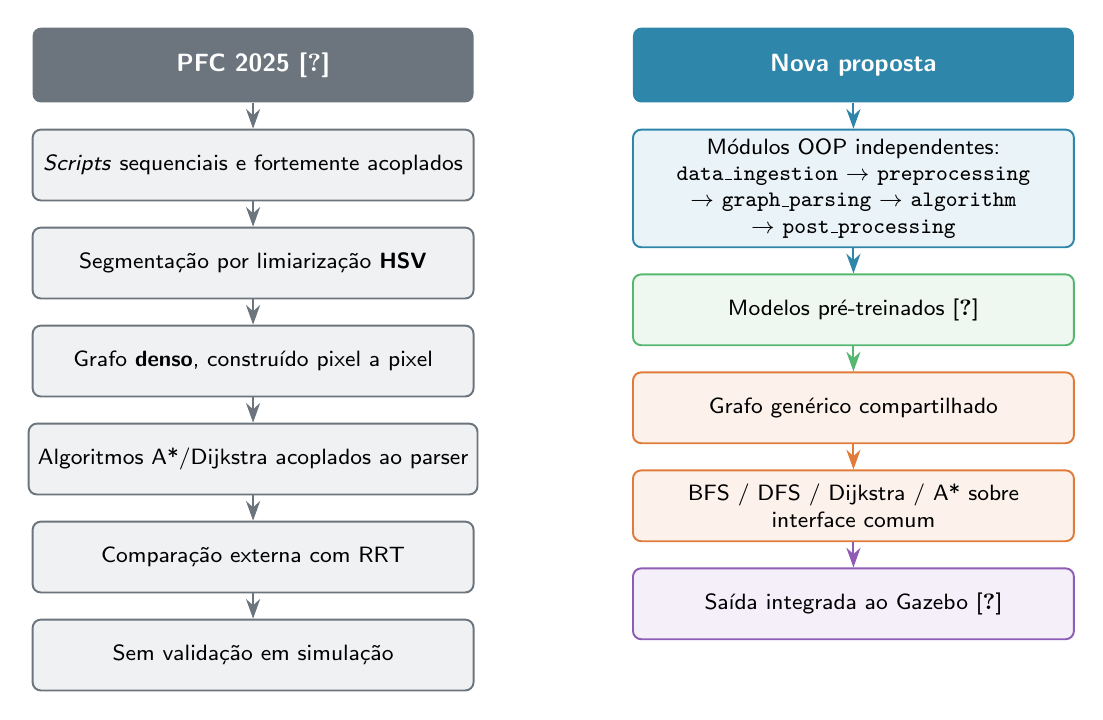
\begin{tikzpicture}[node distance=0.32cm]

        % ════════════════════════════════════════════════════════════════
        %  COLUNA ESQUERDA — PFC 2025
        % ════════════════════════════════════════════════════════════════
        \node[compTitle=boxGray] (tA) {PFC 2025 \cite{camelo2025}};
        \node[compBox=boxGray, below=of tA] (a1)
            {\textit{Scripts} sequenciais e fortemente acoplados};
        \node[compBox=boxGray, below=of a1] (a2)
            {Segmentação por limiarização \textbf{HSV}};
        \node[compBox=boxGray, below=of a2] (a3)
            {Grafo \textbf{denso}, construído pixel a pixel};
        \node[compBox=boxGray, below=of a3] (a4)
            {Algoritmos A*/Dijkstra acoplados ao parser};
        \node[compBox=boxGray, below=of a4] (a5)
            {Comparação externa com RRT};
        \node[compBox=boxGray, below=of a5] (a6)
            {Sem validação em simulação};

        % ── Setas verticais coluna esquerda ──────────────────────────────
        \foreach \src/\dst in {tA/a1, a1/a2, a2/a3, a3/a4, a4/a5, a5/a6}{
            \draw[compArrow=boxGray] (\src) -- (\dst);
        }

        % ════════════════════════════════════════════════════════════════
        %  COLUNA DIREITA — Nova proposta
        % ════════════════════════════════════════════════════════════════
        \node[compTitle=boxBlue, right=2.0cm of tA] (tB) {Nova proposta};
        \node[compBox=boxBlue, below=of tB] (b1)
            {Módulos OOP independentes:\\
             \texttt{data\_ingestion} $\to$ \texttt{preprocessing}\\
             $\to$ \texttt{graph\_parsing} $\to$ \texttt{algorithm}\\
             $\to$ \texttt{post\_processing}};
        \node[compBox=boxGreen, below=of b1] (b2)
            {Modelos pré-treinados \cite{junior2024_models}};
        \node[compBox=boxOrange, below=of b2] (b3)
            {Grafo genérico compartilhado};
        \node[compBox=boxOrange, below=of b3] (b4)
            {BFS / DFS / Dijkstra / A* sobre \\ interface comum};
        \node[compBox=boxPurple, below=of b4] (b5)
            {Saída integrada ao Gazebo \cite{koenig2004}};

        % ── Setas verticais coluna direita ───────────────────────────────
        \draw[compArrow=boxBlue]   (tB) -- (b1);
        \draw[compArrow=boxBlue]   (b1) -- (b2);
        \draw[compArrow=boxGreen]  (b2) -- (b3);
        \draw[compArrow=boxOrange] (b3) -- (b4);
        \draw[compArrow=boxPurple] (b4) -- (b5);

    \end{tikzpicture}}
    \caption{Comparativo da estrutura de código entre o PFC 2025 \cite{camelo2025} e a nova proposta.}
    \label{fig:comparacao_arquitetura}
\end{figure}

\subsection{Plataforma-alvo e Formato de Saída}

A plataforma de execução considerada neste projeto é um UGV simulado no ambiente Gazebo \cite{koenig2004}. O Gazebo é um simulador robótico de código aberto amplamente utilizado na comunidade de robótica, compatível com o \textit{framework} ROS, e permite modelar a dinâmica do veículo, sensores e o ambiente de operação com elevado grau de fidelidade antes da implantação em campo, conforme já discutido na Seção~\ref{sec:gazebo}.

Nesse contexto, o módulo \texttt{post\_processing} é o responsável por produzir uma saída compatível com as entradas esperadas pelo controlador do UGV no Gazebo. O formato adotado é uma sequência de \textit{waypoints}, em que cada ponto contém: coordenadas $(x, y)$ no sistema de referência da imagem, ângulo de proa $\theta$ (orientação para o próximo ponto) e o tipo de movimento associado (translação ou parada). Essa estrutura é encapsulada na dataclass \texttt{RobotPath} e pode ser serializada para os formatos de mensagem ROS (\texttt{nav\_msgs/Path}), permitindo a integração direta com os nós de controle do simulador.

% ── 4.2 ──────────────────────────────────────────────────────────────────
\section{Construção dos Grafos}

A construção dos grafos toma como entrada o mapa de navegabilidade gerado pela segmentação semântica (Seção~\ref{sec:segmentacao}). O parser identifica como nós os pixels marcados como transitáveis e estabelece arestas entre vizinhos imediatos, conforme a conectividade escolhida (4 ou 8 vizinhos). Os principais aprimoramentos em relação ao PFC 2025~\cite{camelo2025} são:

\begin{itemize}
    \item \textbf{Ponderação por transformada de distância}: o peso de cada nó é calculado pela transformada de distância euclidiana (\texttt{scipy.ndimage.distance\_transform\_edt}), substituindo a verificação iterativa pixel-a-pixel do projeto anterior, com ganho substancial de desempenho;
    \item \textbf{Construção vetorizada}: as arestas são construídas de forma vetorizada com operações NumPy, evitando laços Python sobre cada pixel.
\end{itemize}

A função \texttt{build\_grid\_graph()} em \texttt{graph\_parsing/\_grid\_utils.py} é compartilhada entre o \texttt{GridImageGraphParser} (para imagens com cores fixas, como o mapa de navegabilidade adotado em \cite{junior2025_rrt}) e o \texttt{SegmentedImageGraphParser} (para imagens segmentadas semanticamente).

Como possível melhoria a ser avaliada nos próximos experimentos, pretende-se investigar a substituição da matriz de adjacência atual por uma representação em formato CSR (\textit{Compressed Sparse Row})~\cite{saad2003}, por exemplo via \texttt{scipy.sparse.csr\_matrix}. Essa alternativa é, em princípio, atrativa para os grafos de grande porte gerados a partir das imagens utilizadas, mas o impacto efetivo sobre uso de memória e tempo de execução ainda precisa ser medido sobre os mapas reais deste trabalho.

% ── 4.4 ──────────────────────────────────────────────────────────────────
\section{Algoritmos de Planejamento}

Os algoritmos A*, Dijkstra, BFS e DFS foram reimplementados sobre a nova representação de grafo. A lógica comum entre A* e Dijkstra foi extraída para uma função compartilhada \texttt{priority\_queue\_search()}, parametrizada pelo uso ou não de heurística. Os utilitários de reconstrução de caminho e cálculo de custo foram centralizados no módulo \texttt{algorithm/\_utils.py}.

% ── 4.5 ──────────────────────────────────────────────────────────────────
\section{Pós-processamento}

Dois pós-processadores foram implementados:
\begin{itemize}
    \item \texttt{SimpleWaypointProcessor}: converte a sequência de nós em \textit{waypoints} com coordenadas, proa e tipo de movimento, adequados para envio ao sistema de navegação do UGV;
    \item \texttt{ImageDrawingPostProcessor}: desenha os caminhos encontrados sobre a imagem original, com cores distintas por algoritmo e marcadores de início e fim, salvando a imagem anotada em disco.
\end{itemize}

% ── 4.6 ──────────────────────────────────────────────────────────────────
\section{Coleta dos Dados}

Para os experimentos deste projeto, são utilizadas imagens RGB obtidas por drone, de alta resolução, em cenários representativos de operação do UGV (caminhos pavimentados, vegetação, praças e obstáculos diversos). Os modelos de segmentação adotados (Seção~\ref{sec:segmentacao}) já foram treinados em \cite{junior2024_models} sobre o \emph{Semantic Drone Dataset}~\cite{drone_dataset}, e agora serão avaliados no conjunto de imagens obtidos na Quinta da Boa Vista.
% ======================================================================
\chapter{RESULTADOS E DISCUSSÃO}
% ======================================================================

Neste capítulo, apresentamos e discutimos os resultados obtidos nos experimentos realizados com o sistema proposto.

% TODO: Preencher com resultados experimentais detalhados, incluindo:
% - Comparação dos modelos de segmentação de \cite{junior2024_models}
%   (ResNet 50, ResNet 101, EfficientNet-B4, EfficientNet-B5)
% - Porcentagem de área transitável por modelo e por imagem
% - Comparação de algoritmos (A* vs Dijkstra vs BFS vs DFS)
% - Tabelas com métricas: distância, custo, nós explorados, tempo
% - Figuras com caminhos anotados e mapas de navegabilidade
% - Resultados da execução dos waypoints no simulador Gazebo

\section{Comparação dos Modelos de Segmentação}

% TODO: Tabela comparativa entre os modelos pré-treinados de \cite{junior2024_models}
%       (ResNet 50, ResNet 101, EfficientNet-B4, EfficientNet-B5)
%       em termos de mIoU, acurácia, tempo de inferência e qualidade visual
%       do mapa de navegabilidade resultante.

\section{Desempenho dos Algoritmos}

% TODO: Tabelas e figuras com resultados por algoritmo (BFS, DFS, Dijkstra, A*).

\section{Validação no Simulador Gazebo}

% TODO: Apresentar a execução dos waypoints gerados pelo módulo
%       de pós-processamento em um UGV simulado no Gazebo \cite{koenig2004},
%       comentando aderência da trajetória, comportamento dinâmico do veículo
%       e impacto da resolução do grafo na execução final.

% ======================================================================
\chapter{CONCLUSÃO}
% ======================================================================

% TODO: Redigir conclusão completa após obtenção dos resultados

O presente trabalho estendeu o projeto de planejamento de trajetória para robôs terrestres desenvolvido em 2025 \cite{camelo2025}, introduzindo três contribuições principais: uma arquitetura modular orientada a objetos; a adoção de modelos de segmentação semântica especializados em imagens aéreas; e a integração com o simulador Gazebo \cite{koenig2004} para validação dos caminhos gerados.

A arquitetura proposta, organizada em cinco módulos encadeados com interfaces abstratas e fábricas, demonstrou-se flexível e extensível, permitindo a fácil incorporação de novos algoritmos, representações de grafos e métodos de pré-processamento.

A adoção dos modelos pré-treinados disponibilizados em \cite{junior2024_models}, treinados sobre o \emph{Semantic Drone Dataset}~\cite{drone_dataset}, permitiu a geração automática de mapas de navegabilidade no formato consolidado em \cite{junior2025_rrt} a partir de imagens RGB reais de drones, em substituição às abordagens baseadas em segmentação por cor adotadas no projeto anterior.

Por fim, a integração com o simulador Gazebo permitirá validar os \textit{waypoints} gerados em um UGV simulado, fornecendo uma camada adicional de avaliação antes de qualquer implantação em campo.

% ── 6.1 ──────────────────────────────────────────────────────────────────
\section{Perspectivas Futuras}

Apesar das contribuições do presente projeto, ainda permanece como oportunidade para trabalhos futuros a extensão do sistema para o tratamento de \textbf{ambientes dinâmicos}, em que obstáculos podem aparecer, desaparecer ou se mover ao longo da execução, exigindo replanejamento em tempo real do caminho.

% ======================================================================
\chapter{CRONOGRAMA}
% ======================================================================

A Figura~\ref{fig:cronograma}, a seguir, apresenta o cronograma detalhado das atividades realizadas e planejadas ao longo do projeto.

\begin{figure}[H]
    \centering
    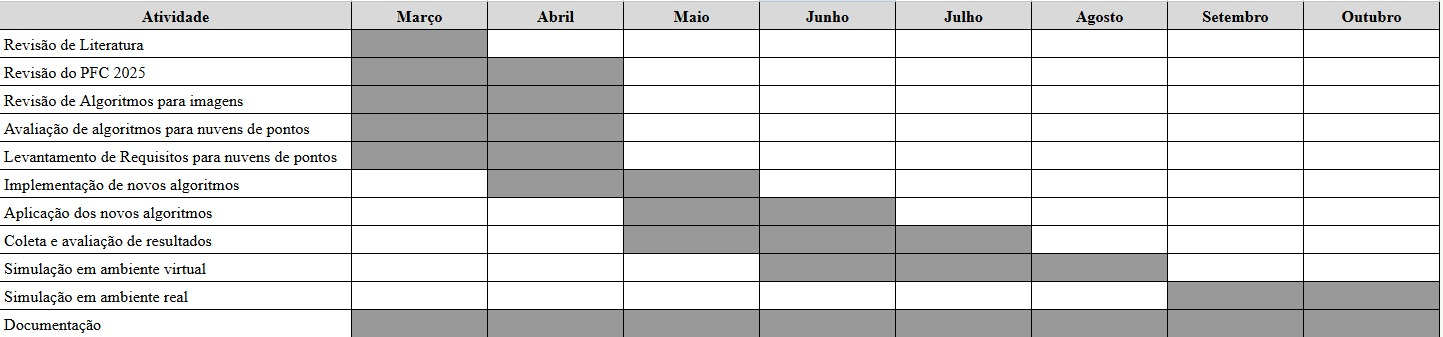
\includegraphics[width=\textwidth]{timeline.png}
    \caption{Cronograma de atividades}
    \label{fig:cronograma}
\end{figure}

% ══════════════════════════════════════════════════════════════════════════
%  REFERÊNCIAS
% ══════════════════════════════════════════════════════════════════════════
\bibliography{referencias}

\end{document}
